\section{Fonction Convertir}

Tous les systèmes physiques ont au moins besoin d'un actionneur pour
agir sur la matière d'œuvre, cet actionneur ne crée pas d'énergie du
néant, il convertit une source d'énergie primaire en énergie adaptée à
l'action souhaitée. Dans le laboratoire les actionneurs seront souvent
des moteurs électriques car cette énergie est directement disponible.



\subsection{Les moteurs électriques}

\begin{center}
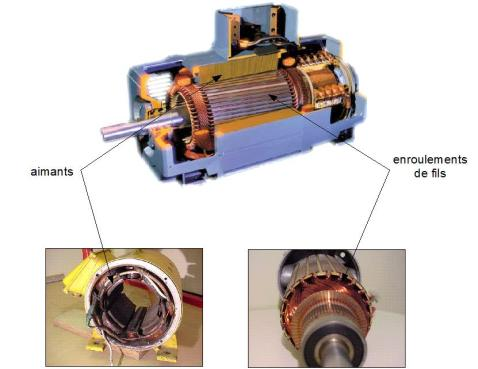
\includegraphics[width=2.91947in,height=2.25279in]{media/image70.jpeg} 
\end{center}

Le moteur électrique est constitué d'aimants et de fils enroulés. Il se
base sur la force de Laplace : tout conducteur parcouru par un courant
et plongé dans un champ magnétique reçoit une force, la force de
Laplace, proportionnelle à l'intensité du courant et du champ
magnétique.

Un système particulier permet de faire varier tourner le champ
magnétique afin de générer une force de Laplace motrice pour le
mouvement de rotation.

Les moteurs électriques sont des machines réversibles, il est possible
de les faire tourner avec un dispositif mécanique pour récupérer une
énergie électrique. On parle de fonctionnement en génératrice. \\

\subsubsection{Le moteur à courant continu}

Les aimants sont liés au stator (partie fixe) et les bobines qui génère
le champ tournant sont liées au rotor. Un dispositif mécanique, les
balais, permettent de faire tourner le champ électrique pour qu'il soit
toujours moteur. Une source de tension continue est suffisante et ce
moteur dispose donc de 2 fil pour l'apport en énergie. Des capteurs
optionnels peuvent augmenter le nombre de connexions.

La modélisation de cet actionneur est détaillée dans un cours. On
observe une proportionnalité du courant avec le couple délivré
(constante de couple Ki) et une proportionnalité de la tension de~force
contre électro motrice~à la vitesse de rotation (constante Ke).
Lorsqu'elles sont exprimées dans un même système d'unité ces constantes
sont proches ou égales.

\subsubsection{Le moteur brushless (sans broches)}

\begin{center}
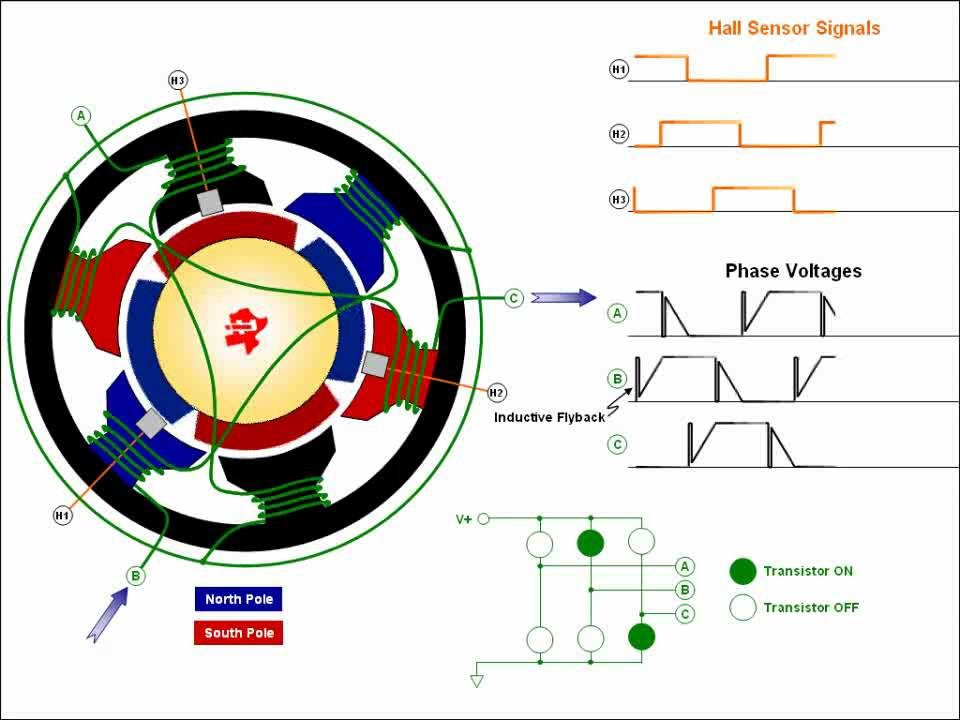
\includegraphics[width=3.79554in,height=2.84745in]{media/image71.jpeg} 
\end{center}

Ce moteur ne dispose pas de dispositif mécanique permettant de faire
tourner le champ. Les aimants sont liés au rotor et 3 connexions
permettent d'alimenter 3 paires de poles (bobines) distinctes. En
alimentant la bonne paire de pole par rapport à la position du rotor
(aimant) le moteur génère un couple positif (il fonctionne).

Afin de choisir la bonne paire de pole il est nécessaire de connaitre la
position du rotor. Un capteur ou des techniques mesurant les courant
d'induction dans les phases permettent de connaitre cette position afin
de piloter le moteur.

\emph{Voir variateur, section «~moduler~»} \\

\subsubsection{Le moteur asynchrone}

Ce type de moteur utilise un champ magnétique dont la vitesse de
rotation n'est pas synchronisée avec la vitesse de rotation. On parle de
glissement. Cette machine est souvent privilégiée notamment pour les
fortes puissances (ferroviaire).

Comme le moteur brushless une électronique de puissance sophistiquée est
nécessaire pour un pilotage performant. Une connexion à un courant
alternatif permettra cependant de la faire tourner sans pilotage.

\subsubsection{Le moteur pas à pas}

\begin{tabular}{ccm{.33\linewidth}}

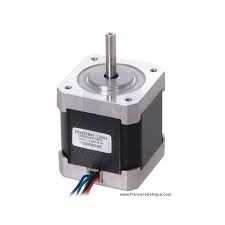
\includegraphics[width=2.0855in]{media/image72.png} &
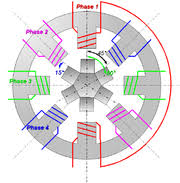
\includegraphics[width=1.875in]{media/image73.png} & Ce
moteur est proche dans son architecture du moteur brushless. Il y a en
plus de poles. Les performances (puissance massique, puissance totale,
efficacité énergétique) sont plus faibles mais le couple est important
ce qui permet de ne pas utiliser de réducteur pour de nombreuses
applications. Aussi chaque pas représente un petit incrément angulaire
ce qui est intéressant pour des activités de précision (pilotage d'un
téléscope de hobbysite, imprimante 3D). \\
\end{tabular}


\subsubsection{Actionneurs linéaires}

Il est possible de faire translater un aimant en le soumettant à un
champ magnétique afin de créer un actionneur linéaire. Ces actionneurs
sont rapides mais l'amplitude possible et la force générées sont en
général limitée. \emph{Exemple~:} prototype d'actionneur de soupapes
pour moteurs sans distribution, prototype de suspensions intelligentes.

La plupart des vérins électrique utilisent en revanche un moteur
électrique tournant associé à un ensemble vis-écrou

\subsection{Convertisseurs d'énergie pneumatique ou hydraulique}


Un vérin est un actionneur utilisant de l'énergie pneumatique ou
hydraulique pour produire une énergie mécanique lors d'un déplacement
linéaire ou rotatif limité à sa course. Le vérin permet de convertir de
l'énergie pneumatique (ou hydraulique) en énergie mécanique.

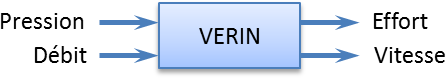
\includegraphics[width=2.9994in,height=0.52326in]{media/image74.png}

Dans les deux cas le produit des deux valeurs donne une puissance, la
puissance \(\mathbf{P \cdot Q}\) pneumatique étant convertie en
puissance \(\mathbf{F \cdot V}\) mécanique. Il est à noter que le
rendement de ces actionneurs est mauvais (\(\eta = 0,5\) environ) : une
grande partie de l'énergie est perdue sous forme d'énergie calorifique
et lors de la mise à l'échappement de l'air comprimé. En prenant en
compte le rendement du compresseur (\(\eta = 0,4\)), on obtient un
rendement global très faible pour la chaîne d'action pneumatique
(\(\eta = 0,2\)). 

\begin{tabular}{cc}
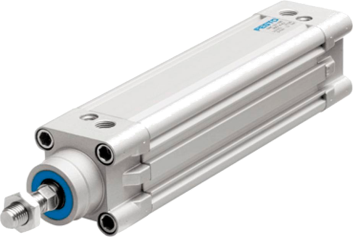
\includegraphics[width=1.60465in,height=1.07872in]{media/image75.png}

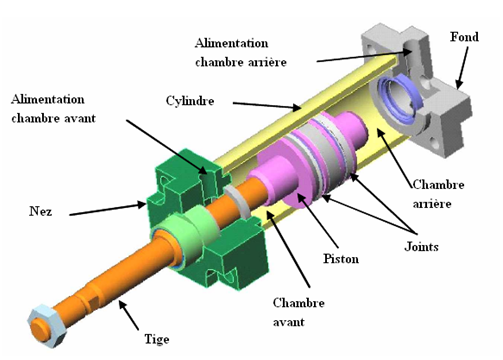
\includegraphics[width=2.54651in,height=1.82389in]{media/image76.png} \\

\end{tabular}

\begin{center}
\begin{tabular}{ccc}
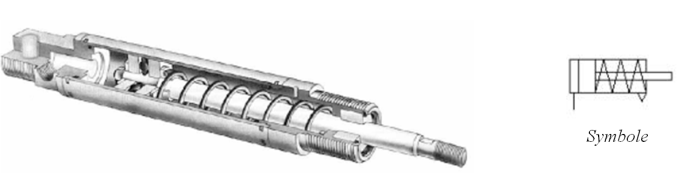
\includegraphics[width=2.18753in,height=0.78785in]{media/image77.png} &
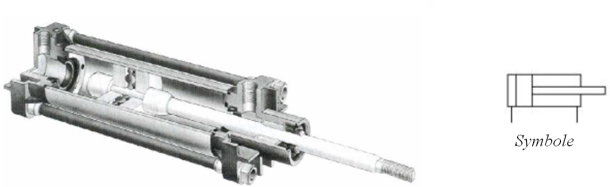
\includegraphics[width=1.94972in,height=0.85305in]{media/image78.png} &
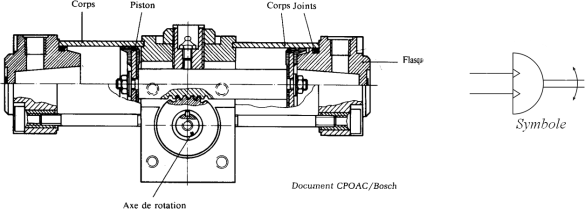
\includegraphics[width=1.95945in,height=0.94776in]{media/image79.png} \\
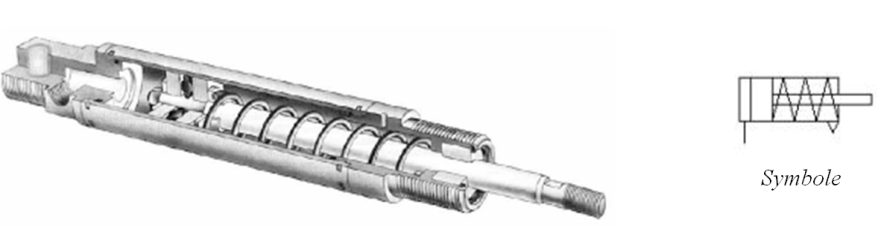
\includegraphics[width=0.7365in,height=0.38835in]{media/image80.png} &
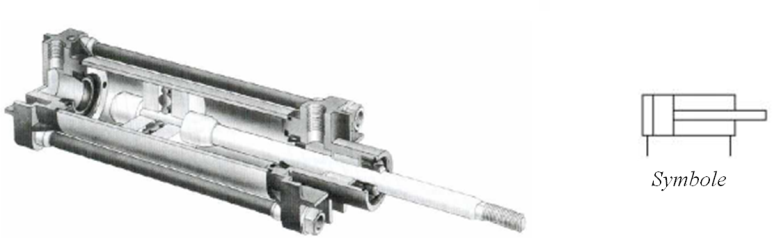
\includegraphics[width=0.68657in,height=0.4208in]{media/image81.png} &
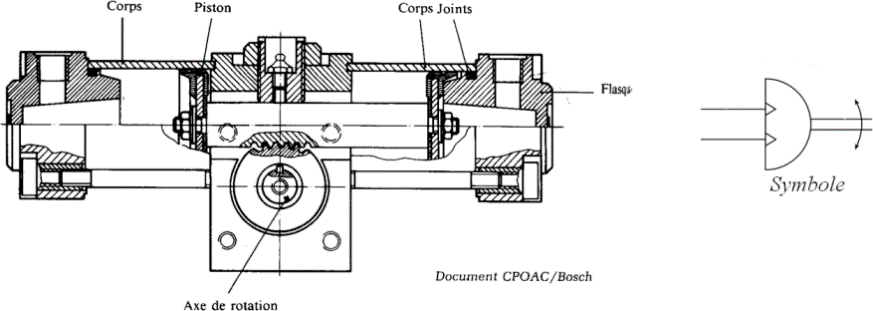
\includegraphics[width=0.83815in,height=0.50289in]{media/image82.png} \\
\emph{\textbf{Vérin linéaire simple effet}} & \emph{\textbf{Vérin
linéaire double effet}} & \emph{\textbf{Vérin rotatif double effet}} \\
\end{tabular}
\end{center}

\textbf{La force} délivrée par un vérin est donnée par \(F = PS\) avec
\(F\) la force en newtons, \(S\) la section du vérin en m² et \(P\) la
pression en Pascals.

\textbf{Le débit volumique} est donné par \(Q = VS\) avec \(Q\) en
m.\textsuperscript{3}s\textsuperscript{-1} et \(V\) la vitesse de
déplacement du vérin en m.s\textsuperscript{-1}.

\textbf{La cylindrée} est donnée par \(C = S\ c\) avec \(S\) en m² et
\emph{c}, la course en m.


\begin{center}
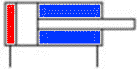
\includegraphics[width=1.42708in,height=0.71875in]{media/image83.png}
\end{center}

On note $D$ le diamètre du vérin et $d$ le diamètre de la tige.

Dans la chambre de gauche l'effort est donné par
\(F_{g} = p_{g}\frac{\pi D^{2}}{4}\).

Dans la chambre de droite l'effort est donné par
\(F_{d} = p_{g}\frac{\pi\left( D^{2} - d^{2} \right)}{4}\). \\


\subsection{Moteurs thermiques}

\begin{center}
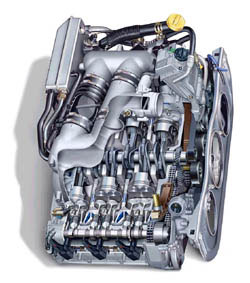
\includegraphics[width=2.79532in,height=3.1643in]{media/image84.jpeg} 
\end{center}

Les moteurs thermiques permettent de récupérer une énergie mécanique, en
général en rotation, à partir d'une source d'énergie chimique. La
combustion peut être externe comme dans une machine à vapeur. Dans un
moteur traditionnel (auto bateau\ldots) ou dans une turbine, un
réacteur, la combustion est interne. Un dispositif mécanique (système
bielle manivelle, ailettes) permet la récupération de l'énergie
mécanique emmagasiné sous forme de pression lors de la combustion. Les
combustions internes sont généralement préférées car elles diminuent les
pertes par échange thermique. Pour aller plus loin~: moteur 4 temps/
moteur 2 temps, cycle Diesel, cycle Beau de Rochas/Otto, moteur rotatif,
distribution.